\documentclass[a4paper,11pt]{article}

\usepackage[utf8]{inputenc}

\usepackage{graphicx}
\usepackage{caption}
\usepackage{subcaption}

\usepackage{pgfplots}
\pgfplotsset{compat=1.18} 

\usepackage{minted}

\begin{document}

\title{
    \textbf{Searching}
}
\author{Edward Sharp}
\date{31-01-25}

\maketitle

\section*{Introduction}

This report investigates and compares the performance differences between linear search and binary search.
A series of experiments are conducted and results are compared, as well as comparing the theory and the order of Ordo between the two methods.


\section*{Linear Search}
\subsection*{Unsorted Search}
When conducting the linear search, the array was made with only positive integers.
To test the worst case scenario of the program the key, the element that is searched for in the array,
was set to $-1$ to ensure that the whole array would be searched and the returned time would be for that of searching the whole array.

\begin{figure}[h!]
  \centering
  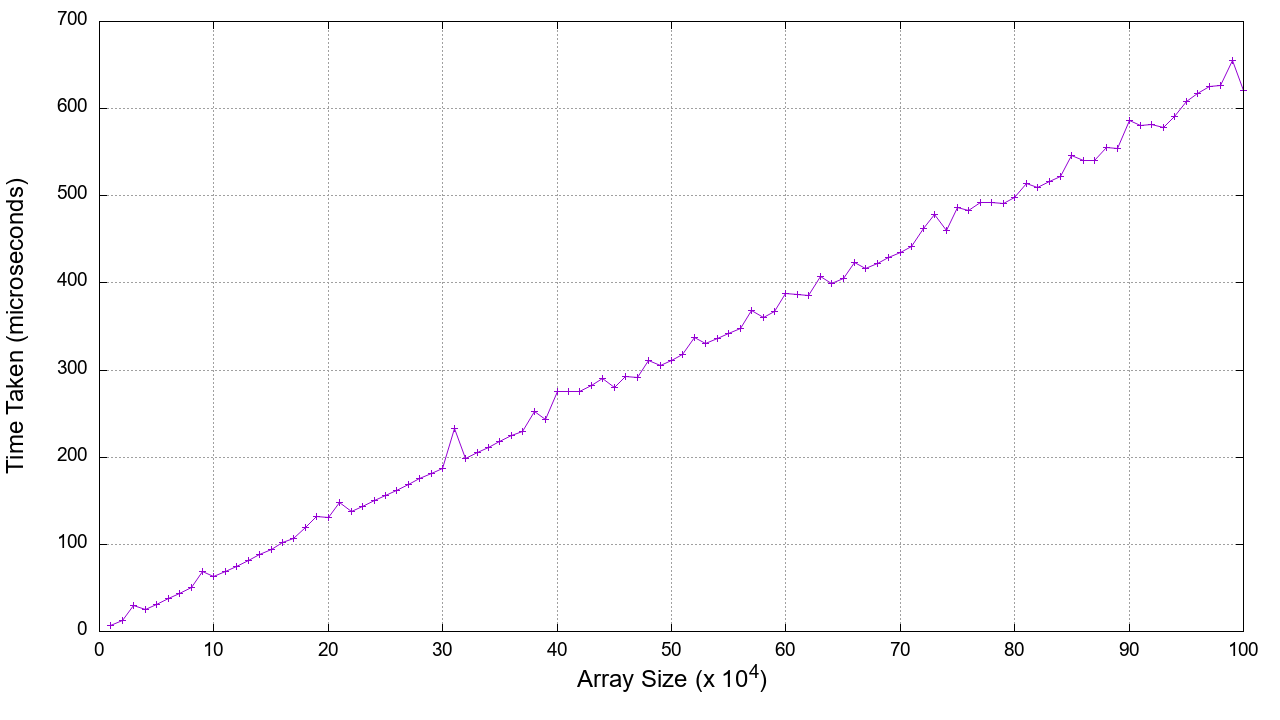
\includegraphics[width=0.8\textwidth]{unsorted_search_plot}
  \caption{Unsorted linear search, array size plotted against time}
  \label{fig:unsorted_search_plot}
\end{figure}

When examining the results found in Figure 1, the linear nature of the algorithms runtime is clearly illustrated.
The time taken the search the array for an element increases linearly with the size of the array, validating the $O(n)$ complexity.

\subsection*{Sorted Search}
For the sorted search, the same procedure for creating the array as for the linear search was done.
In this instance though, two cases were reported; a hit case, and a miss case.
For the miss case, the same procedure as the worst case scenario for the unsorted method was used and reported.
For the hit case, the key was set to the array size divided by two.

\begin{figure}[h!]
  \centering
  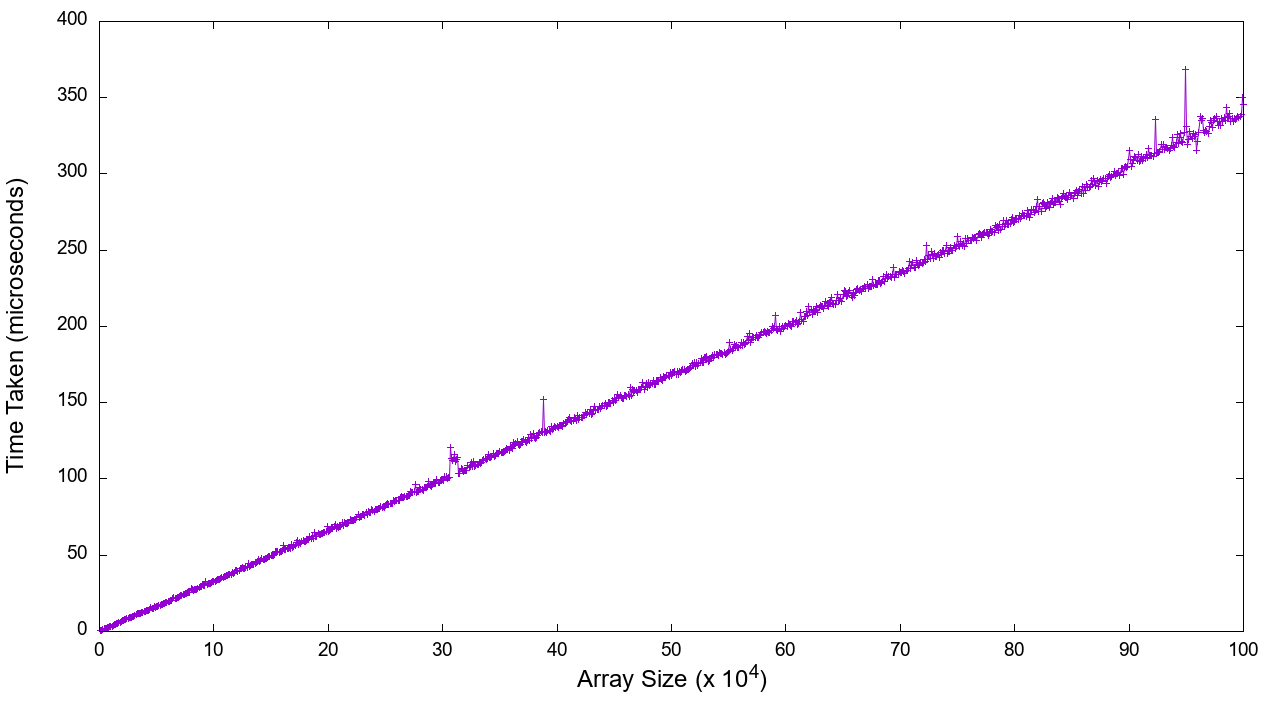
\includegraphics[width=0.8\textwidth]{sorted_search_hit_linear}
  \caption{Sorted linear search, hits, array size plotted against time}
  \label{fig:sorted_search_hit_linear_plot}
\end{figure}

\begin{figure}[h!]
  \centering
  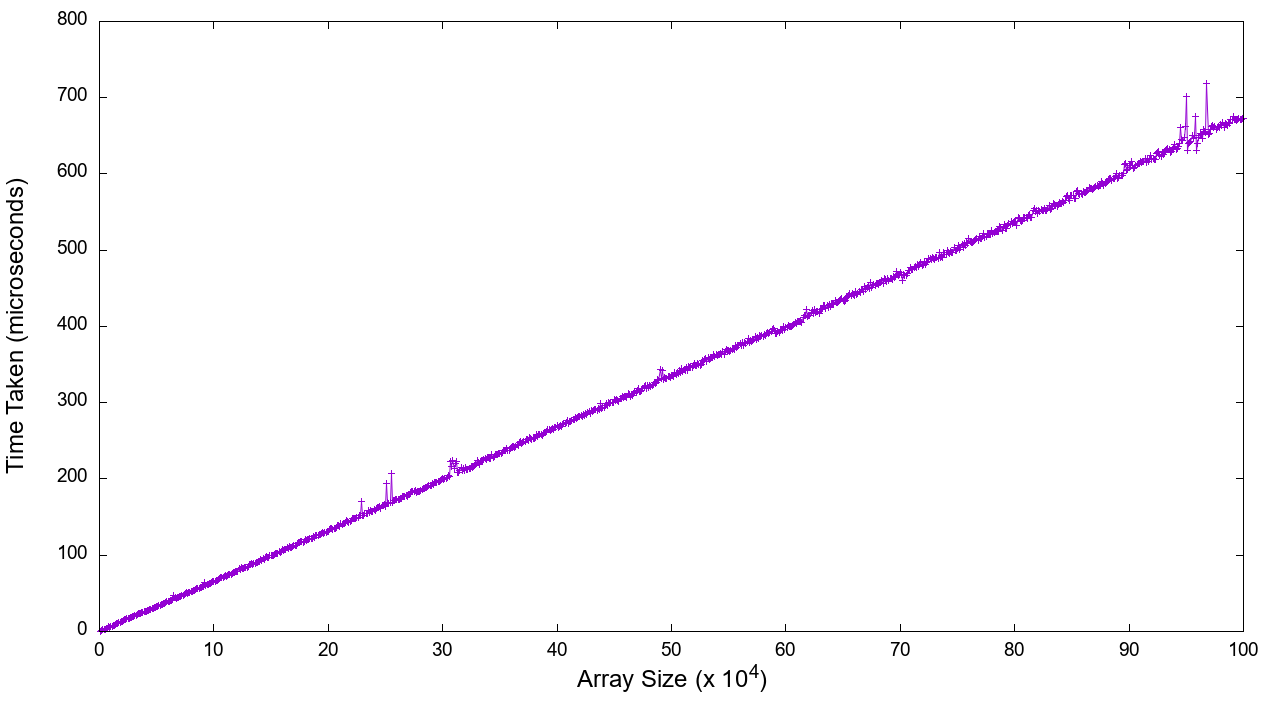
\includegraphics[width=0.8\textwidth]{sorted_search_miss_linear.png}
  \caption{Sorted linear search, misses, array size plotted against time}
  \label{fig:sorted_search_miss_linear_plot}
\end{figure}

As can be seen in Figure 3, compared to Figure 1, the results between the miss case of a sorted search, and that of a search in an unsorted array, is virtually the same.
This is not surprising, since the methods are practically the same as well.
Comparing the hit cases and the miss cases, Figure 2 and Figure 3, it can be seen that the results of the miss cases are consistently rougly half that of the miss cases.
This is also not suprising.
Since this algorithm also expresses the $O(n)$ complexity, being linear, searching half of the array for the hit case would logically take half the time than searching the whole array,
as is done in the miss case.

\section*{Binary Search}
Unlike the linear search, binary search decreases the portion of the array to be searched by half with every iteration.
This is very efficient for sorted arrays, and the time complexity of the worst case scenario expresses a $O(\log(n))$ complexity.
To make the miss case more accurate for this attempt, the key for the miss attempt was set to an arbitrary number, in this case 10,
added to the value of the last element in the array.

\begin{figure}[h!]
  \centering
  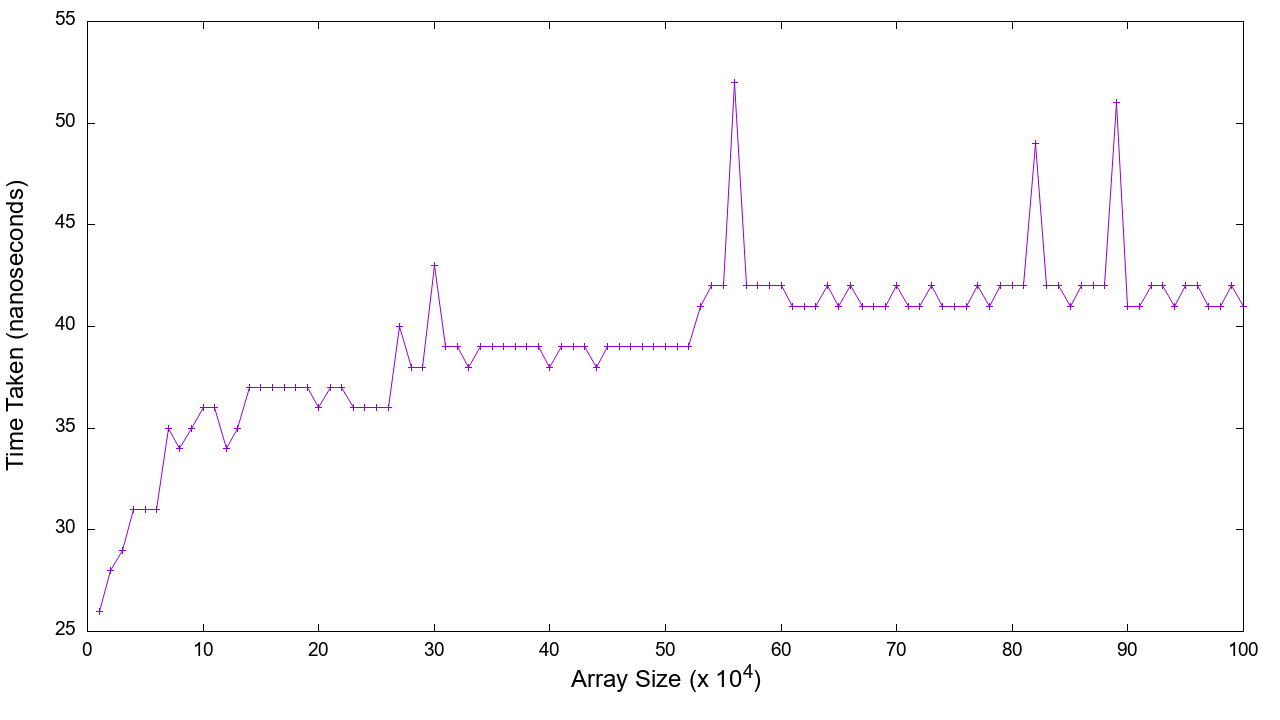
\includegraphics[width=0.8\textwidth]{sorted_search_hit_plot}
  \caption{Sorted binary search, hits, array size plotted against time}
  \label{fig:sorted_search_hit_plot}
\end{figure}

\begin{figure}[h!]
  \centering
  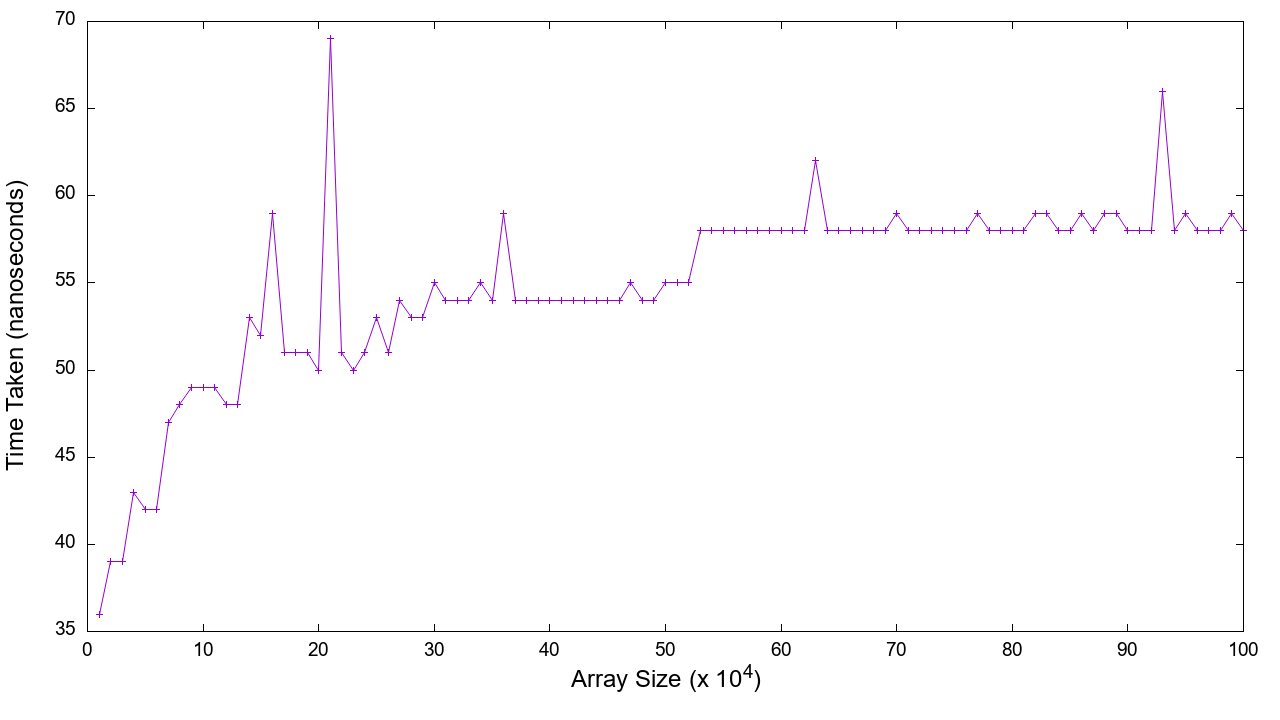
\includegraphics[width=0.8\textwidth]{sorted_search_miss_plot}
  \caption{Sorted binary search, misses, array size plotted against time}
  \label{fig:sorted_search_miss_plot}
\end{figure}

As can be seen from Figure 4 and Figure 5, the binary search is much more efficient than the linear search.
The $O(\log(n))$ complexity can also be seen in the results, but there are some discrepancies in the results seen in the unpredictable spikes at certain points.
Since the execution time is so fast for the binary search, this could be explained by interrupting background activities on the computer occupying computing power.

  Without doing any measurement just now, we could try guessing the expected execution time of a hit case if the array size was $64 \cdot 10^6$.
  Since the complexity is $O(\log(n))$, we could guess that the execution time would not be much more than that of the one millionn array,
  since the curve has already plateaued at that point.
  In testing, the time taken seems to be around 60 nano seconds, a bit more than that of the array with one million elements.

\section*{Conclusion}
This report compared the performances between linear and binary search algorithms on arrays of varying sizes.
The reported results confirmed the theory and expected outcomes from the time complexities involved, $O(n)$ and $O(\log(n))$.
The linear search with a time complexity of $O(n)$ grew much faster in execution time than the binary search,
  with a time complexity of $O(\log(n))$, resulting in much faster execution times for the binary search method, especially when the array size grew larger.
\end{document}
